\documentclass[a4paper]{article}
\usepackage[slovene]{babel}
\usepackage[utf8]{inputenc}
\usepackage[T1]{fontenc}
\usepackage{marvosym}
\usepackage{amssymb,amsmath}
\usepackage{graphicx}
\title{Razvrščanje z dominantnimi množicami}
\author{Taja Debeljak, Anže Marinko \\ Finančni praktikum \\ Finančna matematika, Fakulteta za matematiko in fiziko}
\date{Jesen 2017}

\newtheorem{definition}{Definicija}[section]
\newtheorem{theorem}{Izrek}

\begin{document}
\maketitle
\section{Uvod}
Grupiranje (ang. Clustering) je postopek razvrščanja predmetov znotraj množice v gruče (cluster) tako, da so si predmeti znotraj iste gruče bolj podobni med sabo, kot so si podobni z elementi iz ostalih gruč. \\
Problem združevanja lahko opišemo z uteženim grafom, ki ga definiramo kot trojico $G = (V,E,\omega)$, kjer je $V = {1,\ldots,n}$ končna množica vozlišč, $E \subseteq V \times V$ množica usmerjenih
povezav in $\omega: E \rightarrow \mathbb{R}$ funkcija, ki vsakemu vozlišču dodeli neko vrednost(težo). Vozlišča grafa G ustrezajo predmetom, ki jih je potrebno združevati. \\
Povezave predstavljajo, kateri predmeti so med seboj povezani, utežene povezave pa odražajo podobnosti med povezanimi predmeti. Poleg tega matrika $A_{i,j} = \omega(i,j) \text{ za vse } i, j \in V$ predstavlja podobnost med vozlišči. Imenujemo jo matrika podobnosti. \\
Osnovni lastnosti, ki morata zadostovati gruči, sta:
\begin{itemize}
\item Notranja homogenost: elementi, ki pripadajo gruči si morajo biti med seboj podobni
\item Maksimalnost: gruče ne moremo dodatno povečati z uvedbo zunanjih elementov
\end{itemize}

\begin{definition}
Naj graf G predstavlja primer združevanja množic in naj bo $C \subseteq V$ neprazna podmnožica. \textbf{Povprečna utežena vhodna stopnja} glede na C je definirana kot
$$awindeg_C(i) = \frac{1}{\lvert C \rvert}\sum_{j\in C}A_{i,j}$$
kjer $\lvert C \rvert$ predstavlja velikost množice C. Za $j\in C$ definiramo
$$\phi_C(i,j) = A_{i,j} - awindeg_C(j)$$
Funkcija $\phi_C(i,j)$ je \textit{mera relativne podobnosti} elementa i z elementom j glede na povprečno povezanost elementa i z elementi iz C.\\
\textit{Težo elementa} i glede na množico C definiramo kot
$$W_C(i)=\begin{cases}
1& \text{; če $\lvert C \rvert = 1$},\\
\sum_{j\in C\setminus{i}}\phi_{C\{i\}}(i,j)W_{C\setminus\{i\}}(j)& \text{; sicer}.
\end{cases}$$
Vrednost $W_C(i)$ nam pove koliko podpore prejme element i od elementov $C\setminus\{i\}$ glede na skupno podobnost z elementi iz $C\setminus\{i\}$. Pozitivne vrednosti nam povedo da je i močno
koleriran z $C\setminus\{i\}$.\\
\textit{Skupna teža množice} C pa je definirana z
$$W(C) = \sum_{i\in C}W_C(i)$$
\end{definition}
\begin{definition}{Dominantna množica}\\
Neprazni množici $C \subseteq V$ za katero je $W(T) > 0$ za vsako neprazno množico $T \subseteq C$ pravimo dominantna množica, če velja:
\begin{enumerate}
\item $W_C(i) > 0$ za vse $i \in C$
\item $W_{C\cup\{i\}}(i) < 0$ za vse $i \notin C$
\end{enumerate}
\end{definition}


% dodaj definicijo x^C?

\section{Povezava s teorijo optimizacije}
Če se omejimo na simetrične povezanosti, torej A je simetrična matrika, potem lahko dominantno množico zapišemo kot rešitev naslednjega standardnega kvadratičnega programa
\begin{gather}
max f(x) = x^T A x \\
\text{p. p. } x\in\Delta \subset \mathbb{R}^n
\end{gather}
Kjer je $\Delta = \{x\in\mathbb{R}^n: \sum_{j\in V}x_j = 1 \text{ in } x_j \geq 0 \text{ za vsak } j\in V\}$ standardni simpleks iz $\mathbb{R}^n$.

\section{Povezava s teorijo grafov}
Naj bo $G=(V,E)$ neusmerjen graf, kjer je $V={1,2,\ldots,n}$ množica vozlišč in $E\subseteq V\times V$ množica povezav v grafu. Dve vozlišči $u, v \in V$ sta sosednji, če $(u, v) \in E$. Podmnožici vozlišč $C \subseteq V$ pravimo klika, če so si vsa vozlišča iz te množice med seboj sosedna.\\
Klika C na neusmerjenem grafu F je največja (maximal), če ne obstaja klika D na grafu G, tako da $C \subseteq D$ in $C \not= D$.
\begin{theorem}
Naj bo graf G neusmerjen z matriko sosednosti $A_G$ in naj bo $0 < \alpha < 1$. Vsaka največja klika C grafa G je dominantna množica od $A_\alpha = A_G + \alpha I$. Obratno, če je C dominantna množica od $A_\alpha$ potem je C največja klika v G.
\end{theorem}

\section{Povezava s teorijo iger}
Teorija iger (za razliko od teorije optimizacije) lahko obravnava tudi nesimetrične matrike. Ideja je v zasnovi simetrične igre »clustering game« med dvema igralcema. Akcije V so čiste strategije, ki so na voljo igralcem, matrika A pa predstavlja njihova izplačila. Oba igralca imata popolno znanje o poteku igre in sprejemata neodvisne odločitve o tem katero strategijo bosta izbrala. Matrika izplačil predstavlja prihodke, ki jih dobi igralec če izbere določeno čisto strategijo. Torej, če igralca 1 in 2 uporabita strategijo $(\delta(i),\delta(j))$, kjer je $(i,j)\in V\times V$ potem igralec 1 dobi izplačilo $A_{i,j}$, igralec 2 pa $A_{j,i}$.
Mešana strategija $x\in\Delta$ je verjetnost porazdelitve čistih strategij, ki modelira stohastično strategijo igre nekega igralca. Če igralec 1 in 2 igrata mešani strategiji $(x_1,x_2)\in\Delta\times\Delta$  potem sta pričakovani izplačili igralcev $x_1^TAx_2$ in $x_2^TAx_1$.
Nashevo ravnovesje je profil mešane strategije $(x_1,x_2)\in V\times V$ pri katerem se noben od igralcev ne more povečati svojega izplačila ob nespremenjeni igri drugih igralcev, torej 
$$y_1^TAx_2\leq x_1^TAx_2 \text{ in } y_2^TAx_1\leq x_2^TAx_1$$
Za vse $(y_1,y_2)\in\Delta\times\Delta$. Nashevo ravnovesje je simetrično, če velja $x_1=x_2$. V primeru simetričnega Nashevega ravnovesja se prejšni neenakosti združita v
$$y^TAx\leq x^TAx \text{ za vse } y\in\Delta$$.
Z vidika \textit{clustering game} je simetrično ravnovesje tisto, kjer imata oba igralca enake hipoteze o članstvu v gruči in noben od igralcev ne želi iz gruče. Še več, prejšni pogoj pomeni:
$$\begin{cases}
(Ax)_i=x^TAx; & i\in\sigma(x) \\ (Ax)_i\leq x^TAx; & i\not\in\sigma(x)
\end{cases}$$
ki pa ga lahko interpretiramo kot notranjo homogenost gruče predstavljeno s \textit{podporo x-a} $\sigma(x)$, kjer je $\sigma(x) = \{i\in V; x_i > 0\}$ indeksna množica pozitivnih komponent vektorja x.
Vendar pa Nash ne nujno zagotavlja pogoj maksimuma, kar lahko vseeno zagotovimo z izboljšanjem Nashevega ravnovesja poznanega kot \textit{evolucijsko stabilna strategija (ESS)}. Simetrično Nashevo ravnovesje $x\in\Delta$ je evolucijsko stabilna strategija, če poleg pogoja $y^TAx\leq x^TAx \text{ za vse } y\in\Delta$ zadostuje tudi pogoju $y^TAx= x^TAx \Rightarrow y^TAx<x^TAx \text{ za vse } y\in\Delta\setminus x$.


% popravi to trditev ... glej evolutionary stabile strategies na Wikipediji

\begin{theorem}
Naj bo A matrika podobnosti pri primeru problema združevanja in naj bo $\Gamma$ \textit{clustering game}. Če je C dominantna množica v A, potem je vektor $x^C$ ESS od $\Gamma$. Obratno, če je vektor x ESS od $\Gamma$, potem je $C=\sigma(x)$ dominantna množica od A, če $(Ax)_i\not=x^TAx \text{ za vse } i \not\in C$.
\end{theorem}

\section{Razvrščanje z uporabo dominantnih množic}
Naivna strategija bi lahko bilo oštevilčenje vseh podmnožic $C\subseteq V$ in preverjanje pogojev iz Definicije 1. Ta rešitev je očitno precej neučinkovita, zato si bomo ogledali dve alternativni strategiji. Obe rešitvi izvirata iz teorije iger.

\subsection{Dinamika replikatorjev}
Dinamika replikatorjev (RD) je deterministična dinamična igra, ki je bila razvita v evolucijski teoriji iger. Ta teorija izvira iz zgodnjih sedemdesetih let kot poskus uporabe načel in orodja teorije iger v biološke namene za model evolucije živali. Predvideva idealni scenarij, s katerim so posamezniki ponavljajoč naključno prirejeni iz velike, idealno neskončne, populacije v igro dveh igralcev. V nasprotju s klasično teorijo iger se tukaj igralci naj ne bi obnašali racionalno ali naj ne bi imeli popolnih informacij o igri, ampak delujejo v skladu s podedovanim vedenjskim vzorcem ali čisto strategijo, in domneva se, da zaradi evolucijskega izbora proces sčasoma deluje na porazdelitev vedenja. Splošni razred evolucijskih enačb je podan z naslednjim nizom navadnih diferencialnih enačb:
\begin{gather}
\dot{x}_i = x_i g_i (x)
\end{gather}
za $i = 1,\ldots,n$, kjer je x funkcija odvisna od t (čas).

\subsection{Dinamika okužb in imunizacije}
Dinamika okužb in imunizacije je razred dinamike diskretnega časa, ki je bila uvedena, da bi premagali nekatere računalniške probleme s standardno evolucijsko dinamiko, ki vključujejo dinamiko replikatorjev (RD). Naj omenimo nekaj problemov evolucijske dinamike kot dinamike replikatorjev: ima kvadratno kompleksnost prostora / časa na iteracijo, niso vse stacionarne točke Nasheva ravnovesja, konvergirajo le v limiti po številu iteracij in odkrivanje podpore ravnovesja je nerodno, če se dinamika ustavi pred pravilno konvergenco (tj. po končnem številu korakov).\\
Dinamika okužb in imunizacije je naslednja:
\begin{gather} x(t + 1) = \delta_{S(x)}(x)\lbrack S(x) - x\rbrack + x \end{gather}
kjer smo zapisali x za x (t). Funkcija $S:\Delta\rightarrow\Delta$ je funkcija izbire strategije, ki izpolnjuje naslednje lastnosti:
\begin{gather}
S (x) = \begin{cases}
y & \text{ za nek } y \in \Upsilon (x), \text{ če je } \Upsilon (x) \not= \emptyset, \\
x & \text{sicer,} \end{cases} \end{gather}
kjer $\Upsilon(x)$ predstavlja množico tako imenovanih infektivnih strategij za x in je definirana kot $\Upsilon(x) = \{y \in\Delta : (y - x)^T A x> 0\}$.\\
Odvisno od izbire S(x) v (4) lahko dobimo drugačno dinamiko.\\
Dokler obstaja $y \in\Upsilon (x)$, strategija x ne more biti ravnovesna po definiciji infektivne strategije. Če je temu tako, dinamika (4) meša strategiji x in y (okuži x z y), dokler ne pride do kršitve Nashevih pogojev, ki ga povzroči y, kar se zgodi z upoštevanjem mešalnega faktorja $\delta y (x)$, ki je podan z
\begin{gather}
\delta y (x) =
\begin{cases}
min\{\frac{(x-y)^T A x}{(y-x)^T A (y-x)}, 1\} ,& \text{če} (y - x)^T A (y - x) <0,\\
1, & \text{sicer.}
\end{cases}
\end{gather}
Dinamika okužb in imunizacije prinaša fiksno (ravnovesno) točko, ko je $\Upsilon(x) = \emptyset$. Če je temu tako, je tudi x Nashevo ravnovesje:
\begin{theorem}
Naj bo $x \in\Delta$ strategija. Potem so naslednje izjave ekvivalentne: 
\begin{enumerate}
\item če $\Upsilon(x) = \emptyset$, za x ni infektivne strategije; 
\item x je Nasheva strategija; 
\item x je fiksna (ravnovesna) točka za dinamiko (4).
\end{enumerate}
\end{theorem}
\textbf{Dokaz:} Omejimo se na dinamiko replikatorja. Če se omejimo na simetrične matrike izplačil, imamo povprečno izplačilo strogo naraščajoče vzdolž katere koli nekonstantne poti dinamike okužb in imunizacije: 
\begin{theorem}
Naj bo $\{x(t)\}_t \geq 0$ pot po (4). Torej za vse $t \geq 0$, $u (x (t + 1), x (t + 1)) \geq u (x (t), x (t))$ z enakostjo natanko tedaj, ko $x (t) = x (t + 1)$, pod pogojem, da je matrika izplačila simetrična.
\end{theorem}

\subsection{Iskanje več gruč}
Dinamika replikatorja in dinamika okužb in imunizacije omogočata, da po konvergenci najdemo eno prevladujočo množico. Načeloma je cilj označiti vse dominantne množice za primere težav s problematiko združevanja, vendar je to v splošnem računsko intenzivno, ker imamo lahko eksponentno veliko gruč. V praksi je nedokončana, vendar dobra, pokritost dominantnih množic navadno zadostna za namene uporabe. Najpogosteje uporabljane računske strategije, ki so pomembne za dinamiko okužb in imunizacije, za (delno) označevanje dominantnih množic, so strategija z več začetki, strategija luščenja, tabu-seznam strategije, strategija destabilizacije in druge.

\subsubsection{Strategija z več začetki} Prva strategija je zelo naiva in je sestavljena iz ponovnega zagona dinamike iz različnih, naključnih točk v simpleksu. Ta strategija je učinkovita, če so podatki sestavljeni iz nekaj gruč z velikimi bazeni privlačnosti, tako da je verjetnost vzorčenja točke, ki pripada posameznemu bazenu, relativno visoka. Jasno je, da ni nobenega zagotovila, da bo ta postopek večkrat izpisal iste gruče. Zato je korak po obdelavi namenjen prepoznavanju in izločevanju ponavljajočih se gruč. Strategija z več začetki je dolgoročno optimalna, ker bo na koncu naštela vse dominantne množice, vendar pa lahko zahteva zelo veliko število vzorcev, kar je v praksi neučinkovito.

\subsubsection{Strategija luščenja} Ta strategija sledi drugačni filozofiji in se uporablja predvsem v primerih, ko nas ne zanima iskanje prekrivajočih se gruč. Ideja je spet zelo preprosta in je sestavljena iz iterativnega izvlečenja dominantne množice in odstranitve njenih točk. S tem je očitno zagotovljeno, da se nobena dominantna množica ne bo večkrat pridobivala. Vendar ta strategija ni optimalna, ker je na eni strani število dominantnih množic, ki jih je potencialno mogoče označiti, navzgor omejeno s skupnim številom točk; po drugi strani pa, razen prve dominantne množice, vse naslednje niso nujno dominantne množice prvotnega problema razvrščanja, saj se vsakič, ko so točke dominantne množice odvzete, spremeni osnovni problem združevanja. Kljub pomanjkanju optimnosti je strategija luščenja računalniško privlačna in se jo v praksi uporabljala v številnih aplikacijah.

\subsubsection{Tabu-seznam strategije} Zadnja strategija temelji na dinamiki okužb in imunizacije. Spet bomo preprosto skicirali splošno idejo. Strategija tabu-seznamov sledi cilju nepopolnega nabiranja dominantnih množic, ki so podobne strategiji luščenja, vendar kljub temu zagotavlja dobro pokritost in je brez žrtvovanja optimalne rešitve, kar pomeni, da so izločene gruče dominantne množice prvotnega problema z gručami. Zamisel je ohraniti tabu-seznam med procesom razvrščanja, to je seznamom točk, ki jih ne bi smeli upoštevati med izločanjem dominantne množice. V nekaterih pogledih to počne tudi strategija luščenja, saj so vse točke že izločenih dominantnih množic dodane na tabu-seznam. Vendar, da bi preprečili možnost pridobivanja neveljavnih dominantnih množic, strategija tabu-seznamov preveri veljavnost domnevnih dominantnih množic, ki jih najdemo pod omejitvijo tabu-seznamov. V vsaki dominantni množici izločitvene iteracije je dominantna množica $C \subset V$ ugotovljena z izvajanjem dinamike okužb in imunizacij z naključno inicializacijo z omejitvijo, da ni mogoče uporabiti nobene točke v tabu-seznamu $T \subset V$, to je $C \subseteq V\setminus T$. Ta omejitev preprečuje, da bi bila C veljavna dominantna množica na splošno, to pomeni, da C ne bi bila dominantna množica glede na celotno množico točk V. Da bi preverili veljavnost domnevne dominantne množice C, se dinamika okužb in imunizacij ponovi, inicializira karakteristični vektor $x^C$ in dovoljuje uporabo vseh točk (tudi tistih v tabu-seznamu). Naj bo $C' \subseteq V$ dominantna množica, ki je veljavna, vendar morda ni nova. Obstajata torej dva možna scenarija, v katerih C' lahko štejemo za novo veljavno dominantno množico, ki se doda končnemu rezultatu razvrščanja: $C' \nsubseteqq T$ ali $C' \subseteq T$, toda C' prej še nismo našli.
V prvem primeru se tabu-seznam posodablja z dodajanjem katere koli točke iz $C'\setminus T$ (npr. naključne), medtem ko ostane v prvem primeru tabu-seznam tak, kot je. Če se namesto tega izkaže, da je $C'\subseteq T$, toda je C' že bilo najdeno, zavrnemo C' in dodamo v tabu-seznam katero koli izmed točk iz $V\setminus T$.
Strategija tabu-seznam zagotavlja, da se bodisi veljavna in nova dominantna množica pridobi pri vsaki iteraciji, ali pa se seznam tabu poveča za eno.

\section{Algoritem dinamike okužb in imunizacije s strategijo luščenja}
\texttt{def delta(n):    \# izbira nakjučnega elementa iz simpleksa}\\
\hspace*{1cm}\texttt{return element\_simpleksa(n)}\newline \\
Kjer je element\_simpleksa(n) funkcija, ki vrne naključen vektor dolžine n iz simpleksa, pri čemer je izbira x-a enakomerno porazdeljena na simpleksu.\newline \\
\texttt{def s(x, matrika):  \# izbira strategije y}\\
\hspace*{1cm}\texttt{y = gamma(x, matrika)}\\
\hspace*{1cm}\texttt{if y is None:}\\
\hspace*{2cm}\texttt{return x}\\
\hspace*{1cm}\texttt{return y}\newline \\
Kjer je gamma(x, A) funkcija, ki vrne prvi nakjučen element \texttt{delta(len(x))}, ki zadošča pogoju $(y-x)^TAx > 0$. Če nobeden izmed prvih 10000 naključnih vektorjev ne zadošča temu pogoju, funkcija gamma vrne \texttt{None}.\newline \\

\texttt{def iteracija(x, n):  \# izračun strategije ob času n za začetni vektor (strategijo) x}\\
\hspace*{1cm}\texttt{w = \lbrack x\lbrack i\rbrack  for i in range(len(x))\rbrack }\\
\hspace*{1cm}\texttt{if sum(x) != 0:}\\
\hspace*{2cm}\texttt{ w = \lbrack x\lbrack i\rbrack  / sum(x) for i in range(len(x))\rbrack }

\hspace*{1cm}\texttt{ matrika = \lbrack \lbrack 0 for \_ in range(len(w))\rbrack  for \_ in range(len(w))\rbrack }\\
\hspace*{1cm}\texttt{for i in range(len(w)):}\\
\hspace*{2cm}\texttt{for j in range(len(w)):}\\
\hspace*{3cm}\texttt{if w\lbrack i\rbrack != w\lbrack j\rbrack:}\\
\hspace*{4cm}\texttt{   matrika\lbrack i\rbrack\lbrack j\rbrack = 1 / abs(w\lbrack i\rbrack - w\lbrack j\rbrack)}\\
\hspace*{1cm}\texttt{\# A je matrika podobnosti}\\

\hspace*{1cm}\texttt{pop = w}\\
\hspace*{1cm}\texttt{for \_ in range(1, število iteracij + 1):}\\
\hspace*{2cm}\texttt{strategija = s(pop, matrika)}\\
\hspace*{2cm}\texttt{konstanta = konst\_del(strategija, pop, matrika)}\\
\hspace*{2cm}\texttt{pop = konstanta * (strategija - pop) + pop}\\
\hspace*{1cm}\texttt{return \lbrack w, pop\rbrack }\newline \\
Kjer je konst\_del(y, x, A) funkcija, ki vrne $\delta = (x-y)^TAx/((y-x)^TA(y-x))$, če $\delta<1$ in če $(y-x)^TA(y-x)<-1e-16$, sicer vrne 1.\newline \\

\texttt{x = element\_simpleksa(dolžina vektorja) }\\
\texttt{kor = x }\\
\texttt{gruca = 0 }\\
\texttt{gruce = \lbrack 0 for \_ in range(len(kor))\rbrack }\\
\texttt{while len(kor) > 0: }\\
\hspace*{1cm}\texttt{gruca += 1 }\\
\hspace*{1cm}\texttt{itr = iteracija(kor, n=t\_max) }\\
\hspace*{1cm}\texttt{komp = 0 }\\
\hspace*{1cm}\texttt{for i in range(len(x)): }\\
\hspace*{2cm}\texttt{if gruce\lbrack i\rbrack  == 0: }\\
\hspace*{3cm}\texttt{if itr\lbrack 1\rbrack \lbrack komp\rbrack  > 10 ** (-5/len(kor)**(1/2)) * max(itr\lbrack 1\rbrack ): }\\
\hspace*{4cm}\texttt{gruce\lbrack i\rbrack  = gruca }\\
\hspace*{3cm}\texttt{komp += 1 }\\
\hspace*{1cm}\texttt{kor = \lbrack\rbrack  }\\
\hspace*{1cm}\texttt{for i in range(len(gruce)): }\\
\hspace*{2cm}\texttt{if gruce\lbrack i\rbrack  == 0: }\\
\hspace*{3cm}\texttt{kor.append(x\lbrack i\rbrack ) }\\
\hspace*{1cm}\texttt{if sum(kor) == 0: }\\
\hspace*{2cm}\texttt{kor = \lbrack 1/len(kor) for \_ in range(len(kor))\rbrack  }\\
\texttt{print(gruce) }\newline \\

Navedeni algoritem sva nato pognala na 15 naključno generiranih vektorjih s simpleksa dimenzije 10. Dobljeni rezultat je prikazan na naslednji strani, pri čemer leva navpična črta označuje vrednost 0, desna pa vrednost največje komponente v začetnem vektorju. Ob desnem robu pa je od zgoraj navzdol razporeditev barv gruč od prve proti peti. \\
Opazimo lahko, da je zaradi strategije luščenja le prva (rdeča) gruča zares pravilno združena, druge pa lahko oklepajo kakšno (ali več) izmed pred njo določenih gruč. Predvsem zadnja gruča običajno združuje vse elemente, ki so ostali do konca izven gruč.\\
\center{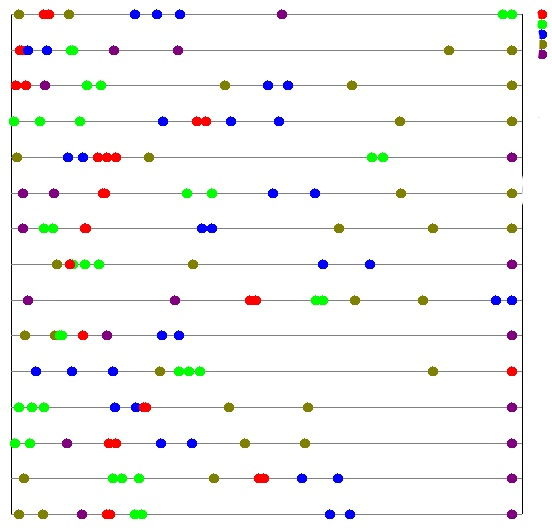
\includegraphics[width=10cm]{dinamika}}\newline \\
\flushleft


% popravi kodo, razlago, bolje opiši algoritem in program ...
% v algoritmu poravi tisto grdo:10 ** (-(20-natancnost)/(4*len(itr[1]))) * max(itr[1])


\section{Zaključek}
V najinem projektu sva se odločila, da za razvrščanje s pomočjo dominantnih množic sprogramirava dinamiko okužb in imunizacije s strategijo luščenja. Dinamika okužb in imunizacije je v najinem primeru iskanje ravnovesja v bimatrični igri $\lbrack A,A^T\rbrack$, kjer je A simetrična matrika podobnosti, kar nas privede do dominantne množice (gruče 1), ki predstavlja množico akcij, med katerimi v ravnovesju meša igralec 1. Z uporabo strategije luščenja pa sicer precej negotovo sestavi še druge gruče.

% Vir!

\end{document}